\section{Photon Detection System Overview}
\label{sec:fdsp-pd-ov}
%\metainfo{(Length: TDR=10 pages, TP=3 pages)}

%%%%%%%%%%%%%%%%%%%%%%%%%%%%%%%%%
\subsection{Introduction}
\label{sec:fdsp-pd-intro}
%\todo{\color{blue} Content: Segreto}

The photon detection (PD) system is an essential subsystem of the DUNE Single-Phase TPC. The detection of the prompt scintillation light signal, emitted in coincidence with an ionizing event inside the active volume, allows the determination of the time of occurrence of an event of interest a thousand times sooner than charge collected from ionization track and with much higher precision. For physics that is uncorrelated with the accelerator, such as proton decay and neutrinos from supernova burst  this information allows determination of the drift time of the ionizing particles.
Knowledge of the drift time provides localization of the event inside the active volume and provides the ability to correct the measured charge for  effects that depend on the drift path length or for specific locations in the detector if there are non-uniformities.  This correction is important for the reconstruction of the energy deposited by the ionizing event, which otherwise would depend on the drift time and on the purity of the liquid argon. In addition to allowing optimum track reconstruction, scintillation light measured by the system could also be used as trigger and for improved calorimetric measurement in combination with charge measurement.

Liquid argon (LAr) is known to be an abundant scintillator and emits about \SI{40}{photons/keV} when excited  by minimum ionizing particles\cite{lar-scint}, in the absence of external electric fields. The passage of ionizing radiation in LAr produces excitations and ionization of the argon atoms that ultimately results in the formation of the 
excited dimer Ar$^*_2$.  Photon emission proceeds through the de-excitation 
of the lowest lying singlet and triplet excited states, $^{1}\Sigma$ and 
$^{3}\Sigma$ to the dissociative ground state. The de-excitation from the 
$^{1}\Sigma$ state is very fast and has a characteristic time of the order of 
$\tau_{fast}$ $\simeq$ 6 ns. The de-excitation from the $^{3}\Sigma$, state is 
much slower with a characteristic time of $\tau_{slow}$ $\simeq$ \SI{1.3}{$\mu$sec}, 
since it is forbidden by the selection rules. 
In both decays, photons are emitted in a \SI{10}{nm} band centered around \SI{127}{nm}, which is in 
the Vacuum Ultra-Violet (VUV) region of the electromagnetic spectrum.
The relative abundance of the  fast and slow components is related to the ionization density of LAr and 
depends on the ionizing particle: \num{0.3} for electrons, \num{1.3} for alpha 
particles and \num{3} for neutrons. This phenomena is the basis for the  
particle discrimination capabilities of LAr exploited by many 
experiments.

In large LAr TPCs, it is common to use {\it photon collector} systems that attempt to 
collect light from large areas and channel it in an efficient way towards  
photosensors that produce an electrical signal.
The paradigm for the detection of LAr scintillation light depends on the use of 
chemical wavelength shifters since most currently available commercial (cryogenic) large area photosensors are not 
directly sensitive to VUV radiation due to the lack of transparency of fused silica and 
glass optical windows. The most widely used wavelength shifter used in 
combination with LAr is Tetra-Phenyl Butadiene (TPB), which absorbs VUV photons 
and re-emits them with a spectrum centered around \SI{430}{nm}, where most of the 
photosensors have their maximum quantum efficiency for photoconversion. 
TPB conversion efficiency is known to be high, there is evidence that 
%, when compared to other wavelength shifters, and 
%it is often taken to be \num{100}\%, even though a reliable direct measurement of this 
%relevant quantity is not available in the literature. 
it approaches 100\% but reliable direct confirmation of this is not available in the literature.

%Scintillation light detection plays several important roles in a LAr TPC such as
%a prompt trigger for potential events of interest and to precisely tag the time of the event, $T_0$, which is needed to 
%determine the absolute position of the event inside the active volume.  It may also allow accurate calorimetric measurement of 
%the deposited energy and so contributes to capability of the TPC as a powerful instrument for particle identification.

Table~\ref{tab:pds-req} summarizes the key performance requirements for the photon detection system.
The first requirement is for minimum light yield of \SI{0.1}{photoelectrons(pe)/MeV} for events that occur near the cathode, which is the farthest region from photon collectors that are embedded in the Anode Plane Assembly (APA) (Chapter\ref{ch:fdsp-apa}). 
The second requirement is that the photon system will provide the timing of events relative to TPC timing, $t_0$, with a 
resolution better than \SI{1}{$\mu$sec}.  The capability to measure the $t_0$ of non-beam events with deposited 
energy above \SI{200}{MeV} will allow observation of proton decay and atmospheric neutrinos with high 
efficiency by enabling 3D spatial localization of candidate events by the TPC. 
The design described in this chapter is motivated by meeting these requirements, however, a consensus has emerged in the collaboration that a revision of these requirements should be considered in order to better exploit the 
characteristics of LAr scintillation light.
% and to improve the performance of the detector for low energy events such as neutrinos from core collapse supernovae. 
There is currently an intense R\&D program to investigate methods to maximize the photon detection efficiency of the PD system within the constraints of the TPC. This will provide two important benefits: the efficiency to identify the interaction time 
(and subsequently improve the calorimetric energy resolution of the interaction through drift-distance correction) is substantially improved at all energies; and, perhaps more importantly, the supernova neutrino tagging efficiency in the region around \SI{20}{MeV} is improved over a larger fraction of the TPC fiducial volume and more robust against uncertainty in the final module performance and manufacturing variations between modules once the light collector efficiency. 

%\fixme{Needs: Performance requirements for the PD system table to expand?}

\begin{dunetable}
[Key performance requirements for the PD system (Note: these are under review).]
%{p{0.8\textwidth}}
{cc}
{tab:pds-req}
{Highest-level PD performance requirements to achieve the detection efficiency of $90$\% for energy deposit of \SI{> 200}{MeV}} 
Requirement  & Value \\ \toprowrule
Light Yield  & \SI{0.1}{pe/MeV} for events near the cathode plane  \\ \colhline
Timing Resolution & \SI{1}{$\mu$s}   \\ \colhline
\end{dunetable}

%%%%%%%%%%%%%%%%%%%%%%%%%%%%%%%%%%%%%
\subsection{Design Considerations}
\label{sec:fdsp-pd-des-consid}
%\todo{\color{blue} Content: Segreto/Warner/Mualem}

The physical dimension of the PD system is constrained by the need to fit within the innermost wire planes of the Anode Plane Assembly (APA) and to be installed through slots in the APA mechanical frame after it is wound (see Section~\ref{sec:fdsp-apa-design}). 
Individual photon detector modules are shaped in the form of thin bars (less than \SI{1}{cm} thick) with approximate dimensions of \SI{8}{cm} $\times$ \SI{200}{cm}. It is anticipated that there will be ten PD modules per APA, for a total of \num{1500} modules. 

%%% rjw 15mar18
%Three different designs of PD modules have been developed and are being 
%considered by the Single-Phase Photon Detector Consortium. Two are based on the concept of 
%light guides coupled to solid state silicon photomultipliers (SiPM) while the 
%third one, namely the ARAPUCA, is functionally a light trap that captures wavelength-shifted photons inside
%boxes with highly reflective internal surfaces where they are eventually detected by an
%SiPM. Figure~\ref{fig:3dtpc-pd} shows a 3-D model of the Single-Phase TPC with a zoom in to the anode plane where the three candidates %photon collector technologies are visible for illustration - in the final detector there will for a single type.
%%%%%%%%%%

%%% rjw 15mar18
\subsubsection{Photon Collectors} 
Three different designs of PD photon collector modules have been developed and are being considered by the Single-Phase Photon Detector Consortium. The baseline design, ARAPUCA\footnote{{\it Arapuca} is the name of a simple trap for catching birds originally used by the Guarani people of Brazil.}, is a relatively new concept that is scalable and has the potential for the best performance of the three designs by a significant factor. It is functionally a light trap that captures wavelength-shifted photons inside boxes with highly reflective internal surfaces where they are eventually detected by a solid state silicon photomultipliers (SiPM).  There are currently two alternative designs based on the use of wavelength-shifters and light guides coupled to SiPMs. Both have undergone more development than ARAPUCA but have performance that meet the physics requirements with only a small safety margin and are not easily scalable within the geometric constraints of the Single-Phase detector.
Figure~\ref{fig:3dtpc-pd} shows a 3-D model of the Single-Phase TPC with a zoom in to the anode plane where the three candidates photon collector technologies are visible for illustration - in the final detector there will be a single type.
%%%%%%%%%%

\begin{dunefigure}[3-D model of photon detectors in the APA.]{fig:3dtpc-pd}
{3-D model of photon detectors in the APA. The model on the left shows the full width of the TPC with the configuration APA-CPA-APA-CPA-APA. The right figure shows a zoom in to the top far side of the TPC where three candidates photon collector technologies are visible for illustration - in the final detector there will be a single type.}
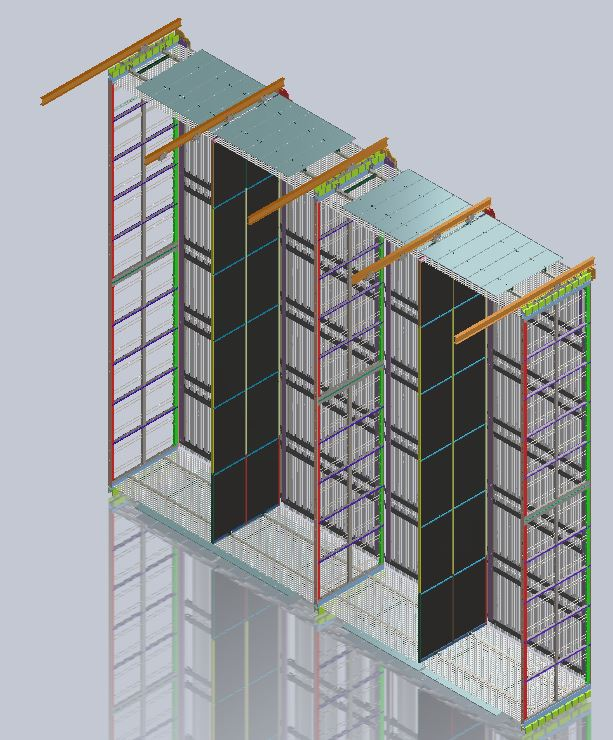
\includegraphics[height=6cm]{pds-dune-sp-tpc-3d.jpg}
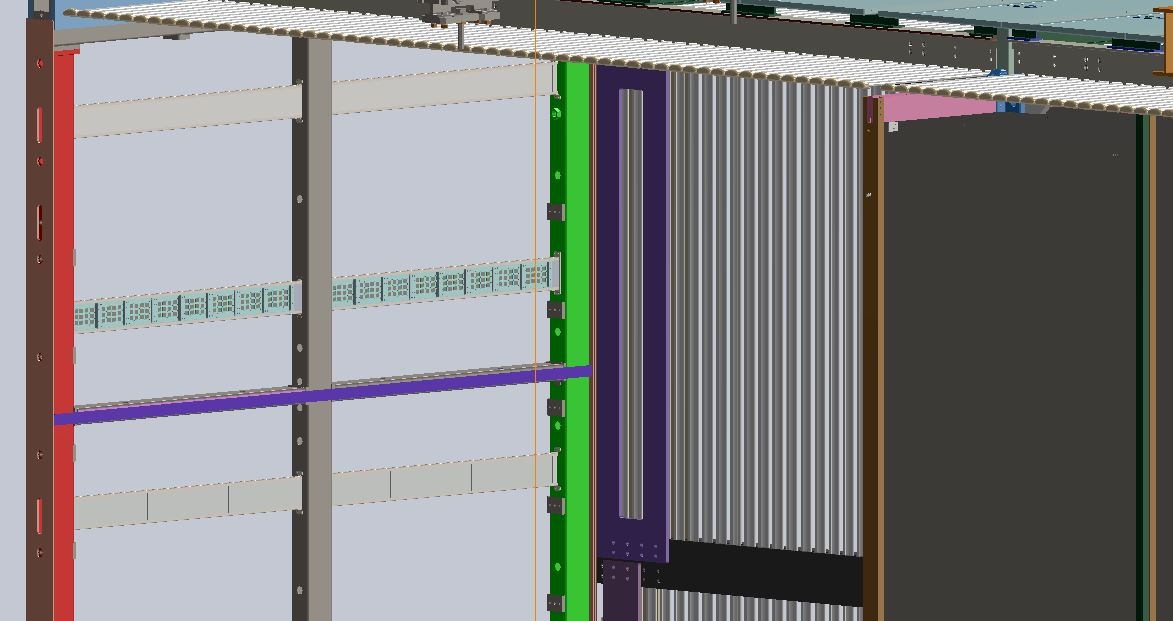
\includegraphics[height=6cm]{pds-dune-sp-tpc-3d-zoom.jpg}
\end{dunefigure}

%DWW 15mar18 start %%%%%%

%The ARAPUCA module is composed of an array of smaller boxes (about \num{20} per module) 
% each one acting as a smaller detector. Each box has an optical window formed  
%by a dichroic filter deposited with two different wavelength shifters, one on 
%the external side and another on the internal one, which allows the light to get
%inside the box, but not to exit. The internal surface of each box is lined 
%with a highly reflective material so that the trapped photon can reflect several 
%times before absorption. An array of SiPMs is installed inside the box to detect the light either 
%directly from the window or after some number of bounces.

The ARAPUCA module is composed of an array of sixteen approximately 8.6$\times$8.6 cm$^2$ boxes, 
 each one acting as an individual detector element, allowing for additional segmentation along the detector bar. 
The initial ARAPUCA collects light from one side through an optical window formed  
by a dichroic filter deposited with a layer of pTP\footnote{p-TerPhenyl,  supplier: Sigma-Aldrich\textregistered}
% https://www.sigmaaldrich.com/catalog/substance/pterphenyl230309294411.} 
wavelength shifter on the external surface that shifts the incident VUV light to a frequency able to pass through the filter plate to the interior of the box.  
In the current version of the device, the inner surface of the box opposite the window houses an array of SiPMs covering a small fraction on the area surrounded by a foil of a highly reflective material coated with another wavelength shifter, TPB\footnote{1,1,4,4-Tetraphenyl-1,3-butadiene, supplier: Sigma-Aldrich\textregistered}. The TPB
%https://www.sigmaaldrich.com/catalog/substance/1144tetraphenyl13butadiene35847145063111},  
converts the light passing through the filter a second time to a wavelength that will be reflected by the filter. It has been shown in simulation and in prototypes that a large fraction of these trapped photons, reflecting from the filter and the lined walls of the box, will eventually fall on an SiPM and be detected.

ARAPUCAs that will be mounted in the central APA frame will need to collect light from both directions. In this case filter plates can be mounted on both sides of the box and the SiPMs moved to the walls.  Here, the second wavelength-shifter (TPB) is coated directly onto the inner surface, but otherwise the double-sided concept functions the same as the one-sided ARAPUCA. 
Another variation under investigation, described in the next section, uses a wavelength-shifter doped plate inbetween the windows.

The ARAPUCA concept is relatively recent -- it was first proposed in 2015 and accepted for installation in ProtoDUNE-SP in mid-2016. A series of tests in LAr have been performed with an evolving prototype design that resulted in efficiency measurements ranging from  \num{0.4}\% to \num{1.8}\%, demonstrating the potential for substantially higher performance than the light-guide designs. Monte Carlo simulations show that efficiencies at the level of few per cent could be reasonably reached with minor modifications to the basic design. 
While the results of the experimental tests are encouraging, a deeper understanding of the optical phenomena utilized by the ARAPUCA concept is needed.

The two solid bars designs have been developed over several years and have reached a reasonable level of maturity and reliability. 
The dip-coated light guides are pre-treated commercially-cut acrylic slabs that are dip-coated with a solution of TPB, acrylic and toluene, when the toluene evaporates it leaves a thin film of TPB embedded in the acrylic matrix.  When LAr scintillation light falls on the bar a fraction of the wavelength-shifted light is captured inside the acrylic bar by total internal reflection and is detected at one or both ends of the bar by an array of SiPMs.
In the double-shift light guides, the conversion and guiding processes of the photons are decoupled. The first conversion is
performed by an ultraviolet transmitting UVT acrylic (radiator) plate coated with pure TPB (through a spraying process) that is positioned \SI{1}{mm} above a commercial doped bar that absorbs the blue light produced by TPB and re-emits it in the green.
 A fraction of the green light propagates down the bar by total internal reflection until it is incident on an
array of SiPM installed at one or both ends. 

Both bar designs have demonstrated attenuation lengths along the long dimension of the bar of the  trapped light comparable to the length of the bars themselves, which ensures a reasonable uniformity along the beam direction. Preliminary measurements indicate an absolute efficiency has been measured to from \num{0.1}\% and possibly as high as  \num{0.4}\%. [Editors note: To be confirmed.]
%Their absolute efficiency has been measured to be in a range between \num{0.1}\% and \num{0.2}\%.
%DWW 15mar18 start %%%%%%
%\fixme{Does IU report efficiency closer to .3 or .4 \%  for the double-dip --email sent to Stu \& Denver}
%DWW 15mar18 end %%%%%%
 Improvements could come from simple extensions of the design such as installing SiPM at both ends of the bars and coating the smaller sides of the bars with reflective foils. 

\subsubsection{Wavelength-shifter Cathode Plane} 
Since the photon detection modules are installed only on the anode plane light collection is not uniform over the entire active volume of the TPC. A possible solution to improve this is to install a reflective foil coated with wavelength shifter on the cathode.
This would increase the light yield of the detector and could enable calorimetric measurements based on light emitted by the ionizing particles. It may also be possible to remove the \Ar39 background through PD-supplied timing cuts, a background that may otherwise cause a huge counting rate for events near  the anode plane. This possibility has yet to be formally adopted by the PD Consortium but is under study through Monte Carlo simulations and the mechanical feasibility is being discussed with the HV Consortium.

%The minimal requirement for the light yield of the PD system is of \SI{0.1}{pe/MeV} 
%near the cathode, which would allow the detector to efficiently  detect ($>$ \num{90}\%) 
%proton decay events (visible energy $>$ \SI{200}{MeV}). All three designs satisfy
%the minimum requirements according to preliminary Monte Carlo 
%studies, but only barely, and there is a consensus inside the Collaboration that a higher 
%light yield would be very beneficial for the detection of low energy supernova 
%neutrinos.  Consequently, a critical review of the requirements is underway.

\subsubsection{Solid State Photosensors} 
In each photon collector concept, the final stage of converting a visible wavelength photon into an electrical signal will be performed by a SiPM. Our experience with a promising early candidate which failed in later batches due to an unadvertised change in SiPM fabrication has emphasized the importance of a multi-source approach where we are actively engaged with potential vendors to develop a device expressly for cryogenic operation. There are ongoing investigations of MPPCs (Multi-Pixel Photon Counter) produced by Hamamatsu (Japan), including one designed for cryogenic operation, and by FBK (Fondazione Bruno Kessler, Italy), which has developed a device for use in the DarkSide cryogenic experiment.

\subsubsection{Readout Electronics} 
For prototype development and for ProtoDUNE-SP, a very capable waveform digitizer has been developed that enables a thorough investigation of the photosensor signals, particularly as we investigate the impact of electrically ganging multiple sensors. The design of the readout electronics for the final system will be strongly influenced by the outcomes of Monte Carlo simulations that are in progress. Of particular interest is the extent to which pulse  shape capabilities are important to maximizing sensitivity to low energy neutrino interactions from supernovae. 
Initial Monte Carlo simulations suggest that it may not be necessary to fully digitize the SiPM waveforms in order to achieve the PD performance requirements.  Charge integration electronic readout systems, which offer the promise of significantly lower cost and and smaller cabling harnesses, are under investigation and is expected to be the baseline solution.
A lower-cost waveform digitization based on lower sampling rate commercial electronics will continue to be investigated as a potential backup option in case our evolving understanding of the requirements necessitates collecting waveform data from the SiPMs.

\subsubsection{R\&D} 
Since the light-guide designs are comparatively well-understood, the need for an improved understanding of the potential ARAPUCA performance drives the strategy for the R\&D program that will be carried out before the Technical Design Report (mid-2019). 
An intense effort is underway to demonstrate that an implementation of the ARAPUCA concept will increase the light yield of the detector by a factor of five to ten with respect to the bars; resources (personnel and funding)  are being sought by the Consortium to achieve this.  
It is anticipated that by the time of the TDR, the Consortium will present ARAPUCA as a baseline design for the photon collector with one alternative design for risk mitigation.  

%DWW 15mar18 end %%%%%%

\subsection{Photon Collection Options Evaluation}
%\todo{\color{blue} Content: Segreto}

The performance of the different photon collection options will be 
evaluated in facilities available to the Consortium that will allow
relative and absolute measurements to be performed at both room and cryogenic temperatures.
The most comprehensive set of data will come from the fully instrumented modules in the ProtoDUNE-SP experiment currently 
under construction at CERN, that will start operations in the last third of \num{2018}.
All  three photon collector designs are present in ProtoDUNE-SP: \num{29} 
double-shift guides, \num{29} dip-coated guides, and two ARAPUCA arrays. The 
presence of the Time Projection Chamber will allow  precise reconstruction
in 3D the track of any ionizing event inside the active volume. The 
matching of the track with the associated light signal will enable an
accurate comparison of the relative detection efficiencies of the different PD 
modules. 
Absolute measurements will be possible depending on the accuracy of the
Monte Carlo simulations of the optical properties of the detector. 
Unfortunately, since some of the optical parameters that 
regulate VUV light propagation in LAr are poorly known, such as Rayleigh 
scattering length, this will influence the precision of the absolute 
measurements. 
%\todo{sounds like we need a plan to measure this somewhere...}

ProtoDUNE-SP will also provide a long-term test of full-scale PD modules for the first time. It will be possible to quantify any deterioration in their performance, which will be important input to determining the necessary initial performance level, such as light yield, that will ensure that the minimal requirements are satisfied for the whole life of the DUNE experiment.

An R\&D program will be executed in parallel with the ProtoDUNE-SP operation since 
additional comparative measurements will be needed, particularly for the newer ARAPUCA concept, prior to establishing the baseline design described in the Technical Design Report.
%DWW 15mar18 start %%%%%%
%The TallBo facility at Fermilab will be extremely important for this program. 
%It provides a \SI{450}{liter} capacity cryostat with \SI{56}{cm} inner diameter and up 
%to a \SI{183}{cm} liquid depth that accommodates  up to three different PD 
%modules with dimensions \todo{how different?} close to the real ones.
% I think we should cut this
%DWW 15mar18 end %%%%%% rjw edits
Several facilities are accessible to the Consortium that will allow testing of smaller scale prototypes of the modules (or secitons of them). 
These include: the ScENE set-up at Fermilab; the cryogenic facilities at Colorado State University and UNICAMP (Brazil); and the optical facilities at Fermilab, Indiana University and UNICAMP.

%DWW 15mar18 start %%%%%%

In addition, PD modules and interfaces with the APA system and cold electronics will be conducted in cryogenic gaseous nitrogen in cold box studies at CERN, utilizing a test stand developed for testing of ProtoDUNE-SP components prior to installation into the detector.  A full-scale ProtoDUNE-SP APA is currently being fabricated, and will be instrumented with cold electronics and photon detectors, allowing the interfaces to be carefully studied.

A small-scale TPC is planned for cold electronics testing at FNAL, and will be instrumented with as many as three 1/2-length PD modules to provide triggering information for the TPC and to continue interface studies with the APA and cold electronics.  It is envisioned that as many as three test cycles will be performed prior to the TDR, allowing testing and continued development of the ARAPUCA concept.
%DWW 15mar18 end %%%%%%
%These facilities will be valuable for the single modules optimization process.

%Timeline appears in the last section.
%A decision on the light collector technology will be made in February 2019.

\subsection{Scope}
\label{sec:fdsp-pd-scope}
%\todo{\color{blue} Content: Segreto/Warner/Mualem}
\fixme{This section is rather "projecty" and doesn't seem to serve any useful purpose - left in since it was part of the original editors template.}

The scope of the photon detector (PD) system for the DUNE far detector 
reference design includes design, procurement, fabrication, testing,
 delivery and installation of the following components:
\begin{itemize}
        \item light collection system;
        \item photosensors (silicon photomultipliers);
        \item readout electronics and cabling;
        \item calibration system (tbd);
        \item (TPB-coated foils for the cathode plane (if implemented));
        \item related infrastructures.
\end{itemize}